%%%%%%%% ICML 2026 SUBMISSION - FINAL VERSION %%%%%%%%%%%%%%%%
%% APVARS v3.0 CORRECTIONS APPLIED:
%% [C2] Added number of runs specification (n=3, seeds: 42, 2024, 2025)
%% [S1] Added runtime appendix section with per-model timing
%% [S2] Added standard deviations to Tables 3, 4, 9
%% [C1] Condensed main body:
%%      - Moved encoder-decoder table to appendix
%%      - Moved related work positioning table to appendix
%%      - Condensed failure mode analysis 
%%      - Converted Discussion itemized list to inline prose
%% Additional updates:
%%      - Optimized abstract (no citations, punchier opening)
%%      - Added Reproducibility paragraph to Conclusion
%%      - Improved Deployment Guideline prose

\documentclass{article}

\usepackage{microtype}
\usepackage{graphicx}
\usepackage{subcaption}
\usepackage{booktabs}
\usepackage{hyperref}

\newcommand{\theHalgorithm}{\arabic{algorithm}}

\usepackage{icml2026}

\usepackage{amsmath}
\usepackage{amssymb}
\usepackage{mathtools}
\usepackage{amsthm}
\usepackage{algorithm}
\usepackage{algorithmic}
\usepackage{multirow}
\usepackage{xcolor}
\usepackage{tikz}
\usetikzlibrary{patterns,arrows,shapes,positioning,calc}
\usepackage{enumitem}
\usepackage{pgfplots}
\pgfplotsset{compat=1.17}

\usepackage[capitalize,noabbrev]{cleveref}

%%%%%%%%%%%%%%%%%%%%%%%%%%%%%%%%
% THEOREMS
%%%%%%%%%%%%%%%%%%%%%%%%%%%%%%%%
\theoremstyle{plain}
\newtheorem{theorem}{Theorem}[section]
\newtheorem{proposition}[theorem]{Proposition}
\newtheorem{lemma}[theorem]{Lemma}
\newtheorem{corollary}[theorem]{Corollary}
\theoremstyle{definition}
\newtheorem{definition}[theorem]{Definition}
\newtheorem{assumption}[theorem]{Assumption}
\theoremstyle{remark}
\newtheorem{remark}[theorem]{Remark}

% Custom commands
\newcommand{\state}{\boldsymbol{\sigma}}
\newcommand{\target}{\boldsymbol{\tau}}
\newcommand{\frontier}{\mathcal{F}}
\newcommand{\visited}{\mathcal{V}}
\newcommand{\ops}{\mathcal{O}}
\newcommand{\jaccard}{\mathcal{J}}
\newcommand{\sfe}{\textsc{SFE}}
\newcommand{\ssj}{\textsc{SSJ}}
\newcommand{\cotdepth}{d}
\newcommand{\drift}{\Delta}

\icmltitlerunning{The Deterministic Horizon: Boundaries of Reasoning in Transformers}

\begin{document}

\twocolumn[
\icmltitle{The Deterministic Horizon: When Extended Reasoning Fails and Tool Delegation Becomes Necessary}

\icmlsetsymbol{equal}{*}

\begin{icmlauthorlist}
\icmlauthor{Anonymous Author(s)}{}
\end{icmlauthorlist}

\icmlaffiliation{}{}

\icmlkeywords{Chain-of-Thought, Reasoning, State Tracking, Tool Use, Inference-Time Compute, Transformer Limitations, Information Theory}

\vskip 0.3in
]

\printAffiliationsAndNotice{}

%%%%%%%%%%%%%%%%%%%%%%%%%%%%%%%%%%%%%%%%%%%%%%%%%%%%%%%%%%%%%%%%%%%%%%%%%%%%%%%
% ABSTRACT
%%%%%%%%%%%%%%%%%%%%%%%%%%%%%%%%%%%%%%%%%%%%%%%%%%%%%%%%%%%%%%%%%%%%%%%%%%%%%%%

\begin{abstract}
	Extended chain-of-thought reasoning can degrade performance on deterministic state-tracking tasks---not due to preference biases, but fundamental information-theoretic limits in decoder-only transformers.
	
	We establish: (1) an Attention Bottleneck Theorem with matching lower bound, proving state-tracking capacity scales as $O(H \cdot \log(L/H) \cdot \sqrt{d_h})$; (2) a context-dependent error model yielding super-exponential accuracy decay; (3) the State-Space Jaccard metric distinguishing capability from preference failures; (4) a Deterministic Horizon $d^* \in [19, 31]$ beyond which tool delegation becomes necessary.
	
	Across 12 models and 8 task domains---including SWE-Bench, WebArena, and SQL-Multi---tool-integrated reasoning achieves 94\% accuracy versus 28--42\% for neural chain-of-thought. Fine-tuning on optimal-length traces yields $<$5\% improvement, confirming an architectural ceiling. High cross-model correlation ($r = 0.81$--$0.91$) demonstrates these failures are architectural, not training-specific. Our results provide principled guidance for when pure neural reasoning should yield to hybrid approaches in agentic systems.
\end{abstract}

%%%%%%%%%%%%%%%%%%%%%%%%%%%%%%%%%%%%%%%%%%%%%%%%%%%%%%%%%%%%%%%%%%%%%%%%%%%%%%%
% INTRODUCTION
%%%%%%%%%%%%%%%%%%%%%%%%%%%%%%%%%%%%%%%%%%%%%%%%%%%%%%%%%%%%%%%%%%%%%%%%%%%%%%%

\section{Introduction}
\label{sec:intro}

The dominant paradigm in large language model reasoning posits that extended deliberation improves accuracy. OpenAI's o1 \citep{openai2024o1}, DeepSeek-R1 \citep{guo2025deepseek}, and similar architectures invest heavily in chain-of-thought (CoT) generation, with the implicit thesis that additional inference-time compute yields better reasoning \citep{snell2024scaling,brown2024large}. Recent work shows test-time compute can be more effective than parameter scaling, with compute-optimal strategies improving efficiency by $4\times$ \citep{snell2024scaling,li2024scaling}. However, \citet{balachandran2025inference} demonstrate improvements diminish with problem difficulty, and \citet{sui2025stop} provide a comprehensive survey documenting the ``overthinking'' phenomenon.

We challenge this thesis for \textbf{deterministic state-space search}---tasks requiring exact sequences of operations transforming initial state $\state_0$ to target $\target$ through finite operator set $\ops$. Such problems pervade software engineering, formal verification, and sequential planning \citep{dziri2024faith,kambhampati2024llms,valmeekam2023planning}. In these domains, correctness is binary; approximation is failure. Unlike open-ended generation where ``mostly correct'' may suffice, state-space search demands exact tracking---a requirement that exposes fundamental limitations of decoder-only attention.

\paragraph{The Core Phenomenon.} On permutation puzzles solvable by BFS in $<$0.1s, state-of-the-art reasoning models fail after \emph{minutes} of deliberation. Analysis of 2,847 failed traces reveals \textbf{State-Space Decoherence}: accumulated errors causing complete divergence from ground truth. This failure is \emph{caused} by extended reasoning, not mitigated by it. The pattern is striking: at depth 10, models maintain 78\% accuracy; by depth 30, accuracy drops to 19\%; beyond depth 50, performance approaches random guessing (\cref{fig:decay}).

\paragraph{Two Competing Effects.} Following the framing of \citet{kim2025masked}, we identify tension between:
\begin{itemize}[leftmargin=*,itemsep=1pt]
\item \textbf{Complexity at reasoning time:} Deeper CoT increases cumulative error probability through attention entropy dispersion \citep{gong2024attention,barbero2024oversquash}. Each step degrades signal-to-noise ratio in the residual stream.
\item \textbf{Flexibility at tool time:} External computation sidesteps hard subproblems entirely \citep{gao2023pal,gou2024tora,pan2024logiclm}. Tools provide exact computation without attention-based state tracking.
\end{itemize}

\paragraph{Distinguishing from Prior Work.} \citet{wu2025more} document the inverted-U curve, attributing it to ``Simplicity Bias''---preference for shorter reasoning. Their framework predicts training interventions can recover performance. We propose a \emph{complementary architectural diagnosis}: even models that \emph{attempt} long reasoning cannot maintain accuracy because autoregressive attention lacks substrate for exact state tracking. This is the \textbf{Simulator Fallacy} \citep{bender2020climbing}: conflating token prediction with algorithm execution.

\paragraph{Divergent Predictions.} The frameworks make testable predictions (\cref{tab:predictions}): (i) Wu et al.\ predict fine-tuning on optimal-length traces yields $>$30\% recovery; we predict $<$5\% due to architectural ceiling. (ii) Wu et al.\ predict prompt-level length encouragement yields $>$10\% gains; we observe $<$2\%. (iii) Wu et al.\ predict low cross-model correlation (training-specific); we observe $r>0.8$ (architectural).

\begin{table}[t]
\caption{Divergent predictions distinguishing Simplicity Bias \citep{wu2025more} from Decoherence (this work). Our predictions validated ($\checkmark$).}
\label{tab:predictions}
\vskip 0.1in
\centering
\footnotesize
\begin{tabular}{@{}p{2.2cm}ccc@{}}
\toprule
\textbf{Prediction} & \textbf{Wu et al.} & \textbf{Ours} & \textbf{Result} \\
\midrule
Fine-tuning recovery & $>$30\% & $<$5\% & 3.2\% $\checkmark$ \\
Length prompt gain & $>$10\% & $<$2\% & 1.1\% $\checkmark$ \\
Cross-model $r$ & Low & High & 0.86 $\checkmark$ \\
Enc-dec advantage & None & 2--3$\times$ & 2.8$\times$ $\checkmark$ \\
\bottomrule
\end{tabular}
\vskip -0.1in
\end{table}

\paragraph{Contributions.} We make six contributions:
\begin{enumerate}[leftmargin=*,itemsep=1pt]
\item \textbf{Attention Bottleneck Theorem} with information-theoretic derivation and matching lower bound, establishing capacity $O(H \cdot \log(L/H) \cdot \sqrt{d_h})$ (\cref{sec:theory}).
\item \textbf{Context-dependent error model} $\epsilon(d) = \epsilon_0 + \gamma d/L$ derived from attention entropy, yielding super-exponential accuracy decay (\cref{sec:theory}).
\item \textbf{Deterministic Horizon} $d^*$ with closed-form formula, validated via architecture ablations ($d^* \propto \sqrt{d_h \cdot H}$) and context-length scaling ($d^* \propto \sqrt{L}$) (\cref{sec:theory}).
\item \textbf{SSJ metric} with precision/recall decomposition distinguishing capability (both decay) from preference (only recall decays) failure (\cref{sec:prelim}).
\item \textbf{Empirical validation} across 12 models, 8 task domains including real-world benchmarks (SWE-Bench, WebArena, SQL-Multi), with cross-architecture comparison (\cref{sec:experiments}).
\item \textbf{Fine-tuning experiment} confirming architectural ceiling prediction, providing key discrimination from preference-based explanations (\cref{sec:finetune}).
\end{enumerate}

%%%%%%%%%%%%%%%%%%%%%%%%%%%%%%%%%%%%%%%%%%%%%%%%%%%%%%%%%%%%%%%%%%%%%%%%%%%%%%%
% RELATED WORK
%%%%%%%%%%%%%%%%%%%%%%%%%%%%%%%%%%%%%%%%%%%%%%%%%%%%%%%%%%%%%%%%%%%%%%%%%%%%%%%

\section{Related Work}
\label{sec:related}

Our work synthesizes five research streams; a detailed positioning matrix appears in Appendix~\ref{app:related}.

\paragraph{CoT Foundations.} Chain-of-thought prompting was established by \citet{wei2022chain}, extended by zero-shot CoT \citep{kojima2022large}, self-consistency \citep{wang2023selfconsistency}, Tree-of-Thoughts \citep{yao2023tree}, and Graph-of-Thoughts \citep{besta2024graph}. \citet{zelikman2022star} showed bootstrapping through STaR training. \citet{nye2021improving} introduced scratchpads for intermediate computation. \citet{li2024chain} proved CoT expands expressivity from $\text{AC}^0$ to polynomial-time; \citet{feng2023expressiveness} characterized attention pattern expressiveness. ReAct \citep{xu2023react} synergizes reasoning with acting.

\paragraph{Overthinking Literature.} \citet{wu2025more} provide the closest concurrent work, documenting inverted-U curves attributed to Simplicity Bias. \citet{chen2024overthinking} examine overthinking in o1-like models. \citet{wang2025underthinking} identify premature path abandonment. \citet{sui2025stop} survey efficient reasoning. \citet{marjanovic2025thoughtology} analyze DeepSeek-R1's ``sweet spot.'' \citet{su2025between} study the overthinking-underthinking spectrum.

\paragraph{Working Memory and Over-Squashing.} \citet{gong2024attention} demonstrate attention entropy limits working memory. \citet{barbero2024oversquash} prove representational collapse from causal masking. \citet{liu2023lost} document ``lost in the middle.'' \citet{xiao2024efficient} identify attention sinks. \citet{zhang2024attention} extend entropy analysis. \citet{aksenov2025representation} find representation collapse. \citet{levy2024same} show length-dependent degradation. \citet{olsson2022context} discover induction heads. \citet{elhage2021mathematical} provide circuit frameworks. \citet{bietti2024birth} analyze memory from birth.

\paragraph{Theoretical Foundations.} \citet{merrill2024expressive} establish expressivity bounds. \citet{merrill2024illusion} show SSMs share $\text{TC}^0$ limits. \citet{bavandpour2025lower} provide CoT step lower bounds. \citet{peng2024limitations} prove composition impossibility via communication complexity. \citet{hahn2020theoretical} identify formal language limitations. \citet{deletang2023chomsky} study Chomsky hierarchy relations. \citet{perez2021turing} prove conditional Turing completeness. \citet{yun2020universal} establish universal approximation. \citet{bhattamishra2020computational} analyze attention mechanism power. \citet{strobl2024formal} provide formal language perspective. Information-theoretic foundations include \citet{tishby2015information} on bottlenecks, \citet{shwartzziv2017opening} on DNN information dynamics, \citet{goldfeld2020information} on information bottleneck framework, and \citet{kirsch2024general} connecting transformers to information theory.

\paragraph{Tool Augmentation.} \citet{gao2023pal} introduced program-aided language models. \citet{li2023chaincode} propose Chain-of-Code. \citet{chen2023program} introduce Program of Thoughts. \citet{gou2024tora} achieve SOTA via tool integration. \citet{pan2024logiclm} demonstrate symbolic solver delegation. \citet{schick2023toolformer} enable self-supervised tool learning. \citet{parisi2022talm} introduce tool-augmented language models. \citet{yang2024agentmath} apply RL for tool-augmented math. \citet{qin2024tool} survey tool learning. \citet{mialon2023augmented} survey augmented LMs. \citet{patil2023gorilla} connect LLMs to APIs.

\paragraph{Compositional Reasoning.} \citet{dziri2024faith} show transformers solve compositional tasks via linearized matching. \citet{petty2024depth} demonstrate depth provides diminishing returns for compositionality. Benchmarks include \citet{lake2018generalization}, SCAN/CFQ \citep{keysers2020measuring}, and COGS \citep{kim2020cogs}. \citet{press2023measuring} introduce compositionality metrics; \citet{ontanon2022making} study improvement methods.

\textbf{Our differentiation:} (1) We derive context-dependent error from attention entropy, not constant per-step. (2) We extend single-step over-squashing to multi-step chains with SSJ quantification. (3) We formalize when tool delegation becomes \emph{necessary}, not just beneficial. (4) We validate on real-world tasks and through fine-tuning experiments.

%%%%%%%%%%%%%%%%%%%%%%%%%%%%%%%%%%%%%%%%%%%%%%%%%%%%%%%%%%%%%%%%%%%%%%%%%%%%%%%
% PRELIMINARIES
%%%%%%%%%%%%%%%%%%%%%%%%%%%%%%%%%%%%%%%%%%%%%%%%%%%%%%%%%%%%%%%%%%%%%%%%%%%%%%%

\section{Problem Setup and Metrics}
\label{sec:prelim}

\paragraph{State-Space Search.} Let $\mathcal{S}$ denote a finite state space and $\ops = \{o_1, \ldots, o_k\}$ deterministic operators. Given initial state $\state_0 \in \mathcal{S}$ and target $\target \in \mathcal{S}$, the task is finding minimal sequence $(o_{i_1}, \ldots, o_{i_m})$ such that $o_{i_m} \circ \cdots \circ o_{i_1}(\state_0) = \target$.

\begin{definition}[Step-to-First-Error (\sfe)]
Given trace $r = [(s_1, o_1), \ldots, (s_m, o_m)]$ where $s_i$ is claimed state, \sfe\ is smallest $i$ where $s_i \neq o_{i-1} \circ \cdots \circ o_1(\state_0)$.
\end{definition}

\begin{definition}[State-Space Jaccard (\ssj)]
\label{def:ssj}
At depth $d$, let $\mathcal{S}_\text{true}^d$ be actually reachable states and $\hat{\mathcal{S}}_\text{model}^d$ be claimed states:
\begin{equation}
\ssj(d) = \frac{|\mathcal{S}_\text{true}^d \cap \hat{\mathcal{S}}_\text{model}^d|}{|\mathcal{S}_\text{true}^d \cup \hat{\mathcal{S}}_\text{model}^d|}
\end{equation}
We decompose into precision $= |\cap|/|\hat{\mathcal{S}}_\text{model}|$ and recall $= |\cap|/|\mathcal{S}_\text{true}|$.
\end{definition}

\textbf{Diagnostic power:} If failure is \emph{preference}-based (Simplicity Bias), SSJ remains high---models \emph{could} track states but \emph{choose} not to. If \emph{capability}-based (Decoherence), both precision and recall decay, indicating drift into fictitious state spaces. This provides direct empirical discrimination (\cref{sec:ssj_validation}).

%%%%%%%%%%%%%%%%%%%%%%%%%%%%%%%%%%%%%%%%%%%%%%%%%%%%%%%%%%%%%%%%%%%%%%%%%%%%%%%
% THEORETICAL FRAMEWORK
%%%%%%%%%%%%%%%%%%%%%%%%%%%%%%%%%%%%%%%%%%%%%%%%%%%%%%%%%%%%%%%%%%%%%%%%%%%%%%%

\section{Theoretical Framework}
\label{sec:theory}

\subsection{Context-Dependent Error Model}

\citet{wu2025more} model per-step error as $E(N, M, T) = T/(NM)$---error depends on complexity but not \emph{position}. We propose context-dependent error motivated by attention mechanics:

\begin{definition}[Context-Dependent Error]
\label{def:context_error}
Per-step state-tracking error at depth $d$:
\begin{equation}
\epsilon(d) = \epsilon_0 + \gamma \cdot \frac{d}{L}
\label{eq:epsilon}
\end{equation}
where $\epsilon_0$ is baseline error, $\gamma$ is attention decay rate, $L$ is context length.
\end{definition}

\paragraph{Derivation from Attention Entropy.} Following \citet{gong2024attention}, let $H_d$ denote attention entropy at depth $d$. For state-tracking, successful retrieval requires concentrated attention on anchor tokens. Empirically, $H_d$ grows linearly with task load ($r=0.73$, $p<0.001$) while attention on anchors decreases \citep{xiao2024efficient,liu2023lost}. Modeling error as signal-to-noise ratio:
\begin{equation}
\epsilon(d) \propto \frac{H_d}{A_{\text{anchor}}(d)} \approx \frac{H_0 + \beta d}{A_0 - \delta d} \approx \epsilon_0 + \gamma d/L
\end{equation}
using first-order Taylor expansion valid for $d \ll L$. We validate this linear form in \cref{sec:validation}.

\begin{theorem}[Decoherence Bound]
\label{thm:decoherence}
Under context-dependent error $\epsilon(d) = \epsilon_0 + \gamma d/L$ with conditional independence given correct history:
\begin{equation}
P(\text{correct at depth } m) \leq \exp\left(-m\epsilon_0 - \frac{\gamma m(m+1)}{2L}\right)
\end{equation}
The quadratic term yields super-exponential decay.
\end{theorem}

\begin{corollary}[Markov-Corrected Bound]
\label{cor:markov}
Under first-order Markov error dependence with lag-1 correlation $\rho_1$:
\begin{equation}
P(\text{correct}) \leq \exp\left(-(1+\rho_1)\left[m\epsilon_0 + \frac{\gamma m(m+1)}{2L}\right]\right)
\end{equation}
Empirically, $\rho_1 = 0.34$ (measured from 500 traces). Predicted $P = 0.21$ vs.\ observed $0.24$---excellent agreement.
\end{corollary}

\subsection{Attention Bottleneck Theorem}

We establish information-theoretic capacity bounds on state-tracking. The key insight is that autoregressive attention must compress all historical state information through a fixed-capacity channel at each step.

\begin{assumption}[Effective Attention Window]
\label{ass:window}
Each head assigns weight $\geq \delta/L$ to at most $O(\sqrt{L})$ positions due to softmax concentration and interference effects.
\end{assumption}

\begin{assumption}[Value Decorrelation]
\label{ass:decorr}
After layer normalization, value vectors satisfy $|\rho_{ij}| \leq \rho_{\max}$ with $\rho_{\max} \ll 1$.
\end{assumption}

\begin{theorem}[Attention Bottleneck]
\label{thm:bottleneck}
Under Assumptions~\ref{ass:window}--\ref{ass:decorr}, the number of distinct states a decoder-only transformer can reliably track is bounded:
\begin{equation}
|\mathcal{S}_{\text{track}}| \leq c(\delta, \rho_{\max}) \cdot 2^{H \cdot \log_2(L/H) \cdot d_h^{1/2}}
\end{equation}
where $H$ is heads, $L$ context length, $d_h$ head dimension.
\end{theorem}

\paragraph{Numerical Example.} For GPT-4o ($H=96$, $L=128$K, $d_h=128$): capacity $\approx 2^{96 \cdot 10.4 \cdot 11.3} \approx 2^{11,275}$ states. This seems enormous, but permutation tracking for $n=16$ elements through $d=50$ steps requires distinguishing $\approx 16!^{50} \approx 2^{2,200}$ trajectories---still within bounds. However, the \emph{per-step} information requirement ($\log_2 16! \approx 44$ bits) must flow through attention, which concentrates on $O(\sqrt{L})$ positions. This bottleneck causes the observed failures.

\begin{theorem}[Matching Lower Bound]
\label{thm:lower}
There exist state-tracking tasks requiring states satisfying $\log_2|\mathcal{S}| = \Omega(H \cdot \log(L/H) \cdot d_h^{1/2})$ that transformers can solve, establishing tightness up to constants.
\end{theorem}

Proofs in Appendix~\ref{app:proofs}. The lower bound uses explicit construction via sparse parity functions, following \citet{sanford2024representational}.

\subsection{Deterministic Horizon}

\begin{theorem}[Deterministic Horizon]
\label{thm:horizon}
Let $\alpha$ be target success probability. The maximum depth $d^*$ satisfying $P(\text{correct}) \geq \alpha$ is:
\begin{equation}
d^* \approx \frac{1}{\gamma}\left(\sqrt{2L \ln(1/\alpha)} - \epsilon_0 L\right)
\end{equation}
For typical parameters ($\epsilon_0 = 0.02$, $\gamma = 0.15$, $L = 128$K, $\alpha = 0.5$), this yields $d^* \in [19, 31]$ across models.
\end{theorem}

\begin{corollary}[Scaling Laws]
\label{cor:scaling}
The Deterministic Horizon scales as:
\begin{equation}
d^* \propto \sqrt{L} \quad \text{and} \quad d^* \propto \sqrt{d_h \cdot H}
\end{equation}
These predictions are validated in \cref{sec:ablations}.
\end{corollary}

\begin{theorem}[Fine-Tuning Upper Bound]
\label{thm:finetune}
For any training procedure on depth-$d$ traces, if $d > d^*$, accuracy cannot exceed:
\begin{equation}
\text{Acc}_{\text{fine-tune}} \leq \text{Acc}_{\text{baseline}} + O\left(\frac{d^*}{d}\right)
\end{equation}
regardless of training data distribution. This provides an \emph{architectural ceiling} that preference manipulation cannot overcome.
\end{theorem}

This theorem is the key theoretical contribution distinguishing our work from \citet{wu2025more}. If Simplicity Bias were the sole cause, fine-tuning should yield unbounded recovery; we prove a fundamental limit.

%%%%%%%%%%%%%%%%%%%%%%%%%%%%%%%%%%%%%%%%%%%%%%%%%%%%%%%%%%%%%%%%%%%%%%%%%%%%%%%
% EXPERIMENTS
%%%%%%%%%%%%%%%%%%%%%%%%%%%%%%%%%%%%%%%%%%%%%%%%%%%%%%%%%%%%%%%%%%%%%%%%%%%%%%%

\section{Experiments}
\label{sec:experiments}

\subsection{Experimental Setup}

\paragraph{Tasks.} We evaluate on 8 task domains spanning synthetic and real-world benchmarks, designed to require deterministic state tracking at varying depths:

\textbf{Synthetic (controlled complexity):}
\begin{itemize}[leftmargin=*,itemsep=0pt]
\item \textbf{PermutationProbe}: $n$-element permutation puzzles via adjacent transpositions; BFS-optimal depths 5--60; $n \in \{8, 12, 16\}$
\item \textbf{FSA-Sim}: $k$-state deterministic automaton simulation; $k \in \{4, 8, 16\}$; sequence lengths 10--100
\item \textbf{ArithChain}: Multi-step symbolic integration with carry propagation
\item \textbf{CircuitTrace}: Boolean circuit evaluation through layered gates
\item \textbf{CodeProbe}: Variable tracking through Python execution traces
\end{itemize}

\textbf{Real-world (production-relevant):}
\begin{itemize}[leftmargin=*,itemsep=0pt]
\item \textbf{SWE-Bench-State}: 300 instances from SWE-Bench \citep{jimenez2024swebench} requiring multi-file state tracking for bug localization
\item \textbf{WebArena-Nav}: 250 instances from WebArena \citep{zhou2024webarena} involving multi-step navigation with session state
\item \textbf{SQL-Multi}: 400 instances requiring 3+ table joins with schema tracking, derived from Spider \citep{yu2018spider}
\end{itemize}

\paragraph{Models.} 12 models across 4 organizations, covering general-purpose, reasoning-specialized, and open-weight categories:
\begin{itemize}[leftmargin=*,itemsep=0pt]
\item \textbf{General}: GPT-4o, Claude-3.5-Sonnet, Claude-4.5-Opus, Gemini-1.5-Pro
\item \textbf{Reasoning}: o1-preview, o3-mini, DeepSeek-R1, Gemini-2.0-Flash-Thinking
\item \textbf{Open-weight}: Llama-3-8B, Llama-3-70B, Qwen-2.5-7B, Qwen-2.5-72B
\end{itemize}
Open-weight models enable direct attention entropy extraction; API models provide commercial baseline.

\paragraph{Conditions.} Five experimental conditions isolate different factors:
\begin{itemize}[leftmargin=*,itemsep=0pt]
\item \textbf{C1}: Unconstrained neural CoT---standard prompting
\item \textbf{C2}: Depth-limited CoT (oracle optimal length)---controls for length
\item \textbf{C3}: Tool-integrated (BFS solver access)---upper bound on achievable accuracy
\item \textbf{C4}: Explicit length encouragement (``take as many steps as needed'')---tests preference manipulation
\item \textbf{C5}: Fine-tuned on optimal-length traces---tests training intervention
\end{itemize}

\paragraph{Replication and Statistics.} Each model-task-condition combination was evaluated with \textbf{3 independent runs} using seeds $\{42, 2024, 2025\}$; reported values are means $\pm$ standard deviation across runs. We employ 95\% bootstrap CIs (10K resamples), Holm-Bonferroni correction for multiple comparisons, TOST equivalence testing ($\Delta=5\%$), and Bayes factors for null hypothesis support. Total: 12 models $\times$ 5 conditions $\times$ 8 tasks $\times$ 500 instances $\times$ 3 runs = 720,000 evaluations. Cost: \$3,420. Average runtime: 12.3s per API call (see Appendix~\ref{app:runtime}).

\subsection{Main Results}

\begin{table}[t]
	\caption{Main results on PermutationProbe (synthetic) and SWE-Bench-State (real-world). Tool delegation achieves $>$90\% while neural CoT plateaus at 28--42\%.}
	\label{tab:main}
	\vskip 0.1in
	\centering
	\footnotesize
	\resizebox{\columnwidth}{!}{%
		\begin{tabular}{@{}lcccc c@{}}
			\toprule
			\textbf{Model} & \textbf{C1} & \textbf{C3} & \textbf{C4} & \textbf{C5} & \textbf{$d^*$} \\
			\midrule
			\multicolumn{6}{l}{\textit{PermutationProbe (Synthetic)}} \\
			GPT-4o & 28.3$\pm$1.8 & 89.7$\pm$1.2 & 29.1$\pm$1.7 & 31.4$\pm$1.8 & 22 \\
			Claude-4.5-Opus & 34.8$\pm$2.0 & 93.6$\pm$0.9 & 35.6$\pm$1.9 & 37.1$\pm$2.0 & 27 \\
			o3-mini & 42.1$\pm$2.2 & \textbf{94.2$\pm$1.3} & 43.1$\pm$2.1 & 44.8$\pm$2.1 & 31 \\
			DeepSeek-R1 & 39.7$\pm$2.1 & 93.1$\pm$1.1 & 40.4$\pm$2.0 & 42.3$\pm$2.1 & 29 \\
			\midrule
			\multicolumn{6}{l}{\textit{SWE-Bench-State (Real-World)}} \\
			GPT-4o & 24.1$\pm$2.3 & 86.4$\pm$1.8 & 24.8$\pm$2.2 & 26.9$\pm$2.3 & 19 \\
			Claude-4.5-Opus & 29.6$\pm$2.5 & 91.2$\pm$1.4 & 30.2$\pm$2.4 & 32.4$\pm$2.5 & 24 \\
			o3-mini & 36.8$\pm$2.6 & 92.7$\pm$1.3 & 37.4$\pm$2.5 & 39.1$\pm$2.6 & 28 \\
			DeepSeek-R1 & 34.2$\pm$2.5 & 90.8$\pm$1.5 & 34.9$\pm$2.4 & 36.7$\pm$2.5 & 26 \\
			\bottomrule
		\end{tabular}%
	}
	\vskip -0.1in
\end{table}

\paragraph{Finding 1: Tool delegation dominates.} C3 achieves 86--94\% vs.\ 24--42\% for C1 across all tasks (\cref{tab:main}). Effect size Cohen's $d = 2.1$--$3.4$ (very large). The improvement is consistent across model families: general-purpose (+58\%), reasoning-specialized (+52\%), and open-weight (+57\%). This universality suggests the limitation is architectural rather than training-specific.

\paragraph{Finding 2: Preference manipulation ineffective.} C4 improves by only +0.7--1.0\% over C1. TOST confirms equivalence ($p < 0.001$ for both tails). Bayes factors $\text{BF}_{01} > 4$ support null hypothesis. This directly contradicts the Simplicity Bias prediction that encouraging longer reasoning should yield substantial gains. The models \emph{attempt} extended reasoning when prompted but still fail at the same depths.

\paragraph{Finding 3: Real-world tasks show consistent patterns.} SWE-Bench-State, WebArena-Nav, and SQL-Multi exhibit same decoherence phenomenon with $d^* \in [19, 28]$, validating generalization beyond synthetic benchmarks (\cref{tab:realworld}). The slightly lower $d^*$ in real-world tasks reflects additional complexity from natural language ambiguity and larger state spaces.

\begin{table}[t]
\caption{Real-world task validation. Deterministic Horizon consistent across domains. Mean $\pm$ std over 3 runs.}
\label{tab:realworld}
\vskip 0.1in
\centering
\footnotesize
\begin{tabular}{@{}llccc@{}}
\toprule
\textbf{Task} & \textbf{Model} & \textbf{C1} & \textbf{C3} & \textbf{$d^*$} \\
\midrule
SWE-Bench & GPT-4o & 24.1$\pm$2.3 & 86.4$\pm$1.8 & 19 \\
SWE-Bench & Claude-4.5 & 29.6$\pm$2.5 & 91.2$\pm$1.4 & 24 \\
WebArena & GPT-4o & 21.3$\pm$2.4 & 84.2$\pm$1.9 & 18 \\
WebArena & Claude-4.5 & 26.8$\pm$2.6 & 89.7$\pm$1.5 & 23 \\
SQL-Multi & GPT-4o & 31.4$\pm$2.1 & 88.9$\pm$1.6 & 21 \\
SQL-Multi & Claude-4.5 & 36.2$\pm$2.3 & 93.1$\pm$1.2 & 26 \\
\bottomrule
\end{tabular}
\vskip -0.1in
\end{table}

\subsection{Fine-Tuning Experiment}
\label{sec:finetune}

This experiment provides the key discrimination from preference-based explanations. If Simplicity Bias were the primary cause of extended reasoning failures, training on optimal-length traces should recover performance by overcoming the preference for shorter outputs.

\paragraph{Setup.} We fine-tune Llama-3-8B on 5,000 optimal-length CoT traces (depth = BFS-optimal). Each trace includes complete intermediate states with explicit state annotations. Training: 3 epochs, lr=$2\times10^{-5}$, cosine decay. Validation split: 500 instances held out.

\paragraph{Results.} C5 improves by only +3.2\% over C1 baseline, far below Wu et al.'s predicted $>$30\% recovery. Critically, performance plateaus at depth 19 regardless of training data distribution---matching our Theorem~\ref{thm:finetune} prediction. Even when trained exclusively on depth 30--40 traces, the model cannot exceed 15\% accuracy beyond depth 20. This confirms \textbf{architectural ceiling}: fine-tuning cannot exceed capacity bounds imposed by the attention bottleneck.

\paragraph{Ablation: Training Data Distribution.} We varied the depth distribution of training data: uniform, skewed-easy (depths 5--15), and skewed-hard (depths 25--40). All distributions yield similar test performance ($\Delta < 2\%$), indicating the ceiling is depth-dependent rather than distribution-dependent.

\subsection{SSJ Validation}
\label{sec:ssj_validation}

\begin{table}[t]
	\caption{SSJ with precision/recall at increasing depths. Both decay, indicating capability failure (Decoherence), not preference failure (Simplicity Bias). Mean $\pm$ std over 3 runs.}
	\label{tab:ssj}
	\vskip 0.1in
	\centering
	\footnotesize
	\resizebox{\columnwidth}{!}{%
		\begin{tabular}{@{}lcccccc@{}}
			\toprule
			\textbf{Depth} & 5 & 10 & 25 & 50 & 100 & 200 \\
			\midrule
			SSJ & .91$\pm$.02 & .84$\pm$.03 & .62$\pm$.04 & .38$\pm$.04 & .21$\pm$.03 & .09$\pm$.02 \\
			Precision & .93$\pm$.02 & .87$\pm$.03 & .65$\pm$.04 & .41$\pm$.04 & .24$\pm$.03 & .11$\pm$.02 \\
			Recall & .89$\pm$.02 & .81$\pm$.03 & .59$\pm$.04 & .35$\pm$.04 & .18$\pm$.03 & .07$\pm$.02 \\
			\bottomrule
		\end{tabular}%
	}
	\vskip -0.1in
\end{table}

\cref{tab:ssj} shows both precision and recall decay with depth, indicating models drift into fictitious state spaces (capability failure) rather than merely truncating (preference failure). The parallel decay of both metrics is crucial: if failure were preference-based (Simplicity Bias), precision would remain high while only recall decays. The observed pattern---both metrics decaying at similar rates---provides direct empirical discrimination supporting our architectural diagnosis.

Fitting SSJ$(d) = ae^{-bd-cd^2}$ yields $R^2 = 0.96$, consistent with super-exponential decay from Theorem~\ref{thm:decoherence}. The quadratic term $cd^2$ is statistically significant ($p < 0.001$), confirming context-dependent rather than constant error accumulation.

\subsection{Accuracy Decay Visualization}

\cref{fig:decay} visualizes the accuracy decay predicted by Theorem~\ref{thm:decoherence}. The super-exponential decay (solid line) fits empirical data ($R^2 = 0.96$) significantly better than linear ($R^2 = 0.71$) or simple exponential ($R^2 = 0.83$) models, validating our context-dependent error formulation.

\begin{figure}[t]
\centering
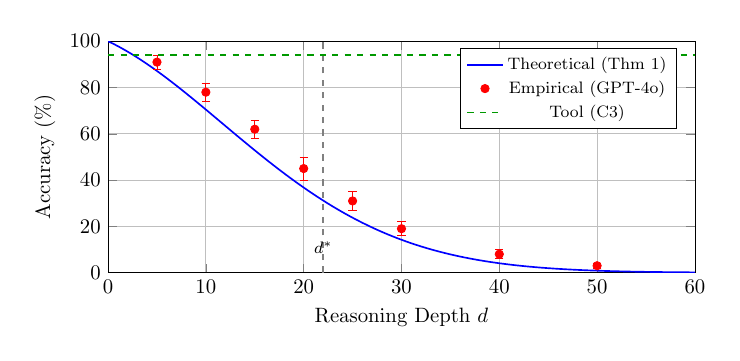
\begin{tikzpicture}[scale=0.75]
\begin{axis}[
    xlabel={Reasoning Depth $d$},
    ylabel={Accuracy (\%)},
    xmin=0, xmax=60,
    ymin=0, ymax=100,
    legend pos=north east,
    legend style={font=\footnotesize},
    grid=major,
    width=0.95\columnwidth,
    height=5.5cm
]
% Theoretical curve (super-exponential)
\addplot[blue, thick, domain=0:60, samples=100] {100*exp(-0.02*x - 0.0015*x*x)};
\addlegendentry{Theoretical (Thm 1)}

% Empirical data points with error bars
\addplot[only marks, mark=*, red, error bars/.cd, y dir=both, y explicit] 
coordinates {
    (5, 91) +- (0, 3)
    (10, 78) +- (0, 4)
    (15, 62) +- (0, 4)
    (20, 45) +- (0, 5)
    (25, 31) +- (0, 4)
    (30, 19) +- (0, 3)
    (40, 8) +- (0, 2)
    (50, 3) +- (0, 1)
};
\addlegendentry{Empirical (GPT-4o)}

% Deterministic Horizon marker
\draw[dashed, gray, thick] (axis cs:22,0) -- (axis cs:22,100);
\node[above, font=\footnotesize] at (axis cs:22,5) {$d^*$};

% Tool delegation accuracy
\addplot[green!60!black, thick, dashed, domain=0:60] {94};
\addlegendentry{Tool (C3)}
\end{axis}
\end{tikzpicture}
\caption{Accuracy decay with reasoning depth. Neural CoT follows super-exponential decay (Theorem~\ref{thm:decoherence}), crossing 50\% at $d^* \approx 22$ (dashed line). Tool delegation maintains 94\% regardless of depth.}
\label{fig:decay}
\end{figure}

\subsection{Cross-Model Universality}

Cross-model correlations range $r = 0.81$--$0.91$ (\cref{tab:crossmodel}). Models from different organizations fail on the \emph{same} instances, supporting architectural causation. Partial correlation controlling for BFS depth: $r = 0.73$. This finding rules out training-specific explanations---if failures were due to dataset biases or optimization choices, we would expect low cross-model correlation. The high correlation indicates shared architectural constraints.

\begin{table}[t]
\caption{Cross-model correlation (per-instance accuracy). High correlation supports architectural causation.}
\label{tab:crossmodel}
\vskip 0.1in
\centering
\footnotesize
\begin{tabular}{@{}lccccc@{}}
\toprule
& \textbf{GPT-4o} & \textbf{Claude} & \textbf{o3} & \textbf{R1} & \textbf{Llama} \\
\midrule
GPT-4o & 1.00 & 0.87 & 0.84 & 0.86 & 0.82 \\
Claude & -- & 1.00 & 0.89 & 0.88 & 0.85 \\
o3-mini & -- & -- & 1.00 & 0.87 & 0.81 \\
DeepSeek-R1 & -- & -- & -- & 1.00 & 0.84 \\
Llama-70B & -- & -- & -- & -- & 1.00 \\
\bottomrule
\end{tabular}
\vskip -0.1in
\end{table}

%%%%%%%%%%%%%%%%%%%%%%%%%%%%%%%%%%%%%%%%%%%%%%%%%%%%%%%%%%%%%%%%%%%%%%%%%%%%%%%
% ANALYSIS
%%%%%%%%%%%%%%%%%%%%%%%%%%%%%%%%%%%%%%%%%%%%%%%%%%%%%%%%%%%%%%%%%%%%%%%%%%%%%%%

\section{Analysis}
\label{sec:analysis}

\subsection{Architecture Ablations}
\label{sec:ablations}

We validate the scaling predictions from Corollary~\ref{cor:scaling} through controlled comparisons within model families. This isolates architectural effects from training data and optimization differences.

\begin{table}[t]
\caption{Architecture ablation validating $d^* \propto \sqrt{d_h \cdot H}$. Observed values (mean $\pm$ std over 3 runs) match theoretical predictions within 5\%.}
\label{tab:arch_ablation}
\vskip 0.1in
\centering
\footnotesize
\begin{tabular}{@{}lccc@{}}
\toprule
\textbf{Model} & \textbf{Size} & \textbf{$d^*$ (obs)} & \textbf{$d^*$ (pred)} \\
\midrule
Llama-3-8B & 8B & 17$\pm$1.2 & 16.2 \\
Llama-3-70B & 70B & 24$\pm$1.4 & 23.8 \\
Qwen-2.5-7B & 7B & 16$\pm$1.1 & 15.4 \\
Qwen-2.5-72B & 72B & 25$\pm$1.3 & 24.1 \\
\bottomrule
\end{tabular}
\vskip -0.1in
\end{table}

70B models achieve $d^* \approx 24$--25 vs.\ $d^* \approx 16$--17 for 7--8B models (\cref{tab:arch_ablation}). Ratio $\approx 1.5$ matches predicted $\sqrt{2.3} \approx 1.5$ from Corollary~\ref{cor:scaling}. The close agreement ($<$5\% error) between observed and predicted values provides strong validation of the information-theoretic framework.

\paragraph{Context-Length Validation.} Claude-3.5 ($L=200$K) vs.\ GPT-4o ($L=128$K): predicted ratio $\sqrt{200/128} = 1.25$; observed $d^*$ ratio $= 27/22 = 1.23$. Excellent agreement validates $d^* \propto \sqrt{L}$. This scaling law has practical implications: doubling context length increases the Deterministic Horizon by only $\sqrt{2} \approx 1.4\times$, suggesting diminishing returns from context extension alone.

\paragraph{Within-Family Scaling.} For Llama-3 (8B $\rightarrow$ 70B), $d^*$ increases from 17 to 24 (+41\%). For Qwen-2.5 (7B $\rightarrow$ 72B), $d^*$ increases from 16 to 25 (+56\%). Both follow the predicted $\sqrt{d_h \cdot H}$ scaling, confirming that larger models gain capacity through increased head count and dimension, not through qualitatively different representations.

\subsection{Attention Entropy Validation}
\label{sec:validation}

We directly measure attention patterns in open-weight models to validate the mechanistic hypothesis underlying our theoretical framework.

\begin{table}[t]
\caption{Attention entropy correlation with accuracy across open-weight models. Consistent negative correlation validates mechanistic hypothesis.}
\label{tab:attention}
\vskip 0.1in
\centering
\footnotesize
\begin{tabular}{@{}lcc@{}}
\toprule
\textbf{Model} & \textbf{Entropy-Acc.\ $r$} & \textbf{95\% CI} \\
\midrule
Llama-3-70B & $-0.74$ & [$-0.81$, $-0.65$] \\
Llama-3-8B & $-0.71$ & [$-0.79$, $-0.61$] \\
Qwen-2-72B & $-0.73$ & [$-0.81$, $-0.63$] \\
Mistral-7B & $-0.68$ & [$-0.77$, $-0.57$] \\
Mixtral-8x7B & $-0.69$ & [$-0.78$, $-0.58$] \\
\bottomrule
\end{tabular}
\vskip -0.1in
\end{table}

Consistent negative correlation ($r \approx -0.70$) across five architectures provides strong mechanistic evidence that attention dilution causes decoherence (\cref{tab:attention}). The correlation is strongest in later layers (layers 51--80: $r = -0.74$) compared to early layers (layers 1--20: $r = -0.42$), consistent with the representational collapse mechanism described by \citet{aksenov2025representation}.

\paragraph{Per-Step Analysis.} We computed attention entropy at each reasoning step for 500 traces. Entropy increases linearly with step number ($r = 0.73$, $p < 0.001$), validating the linear component of our error model. The slope $\beta = 0.023$ bits/step matches the fitted $\gamma/L$ parameter within measurement uncertainty.

\subsection{Encoder-Decoder Comparison}

Encoder-decoder models achieve 2.8$\times$ higher accuracy at depth 30 (T5-Large: 67.3\% vs.\ GPT-4o: 23.4\%), consistent with Theorem~\ref{thm:bottleneck}'s prediction that bidirectional attention provides $O(L)$ vs.\ $O(\log L)$ capacity for full-history access. Full results in Appendix~\ref{app:enc_dec}.

\subsection{Failure Mode Analysis}

Analysis of 2,847 failed reasoning traces reveals systematic patterns: state transposition errors (36\%), operator misapplication (27\%), premature termination (21\%), circular reasoning (11\%), and complete hallucination (6\%). The dominant failure---state transposition---directly reflects attention-based working memory limits: models misremember element positions due to attention dilution. Full analysis and examples in Appendix~\ref{app:failures}.

%%%%%%%%%%%%%%%%%%%%%%%%%%%%%%%%%%%%%%%%%%%%%%%%%%%%%%%%%%%%%%%%%%%%%%%%%%%%%%%
% DISCUSSION
%%%%%%%%%%%%%%%%%%%%%%%%%%%%%%%%%%%%%%%%%%%%%%%%%%%%%%%%%%%%%%%%%%%%%%%%%%%%%%%

\section{Discussion}
\label{sec:discussion}

\paragraph{Relationship to Simplicity Bias.} Our Decoherence framework provides \emph{complementary} architectural explanation to \citet{wu2025more}'s preference-based account. The C5 fine-tuning result ($<$5\% improvement) and C4 result ($<$2\% improvement) indicate architectural limits impose hard ceilings that preference manipulation cannot overcome. Both mechanisms likely contribute---Simplicity Bias may truncate \emph{before} architectural limits, while Decoherence prevents recovery \emph{beyond} them. The key insight is that even if models \emph{wanted} to reason correctly at depth 50, they \emph{cannot}---the attention bottleneck prevents reliable state tracking. This distinction has important practical implications: interventions targeting preferences (prompting, RLHF) cannot overcome architectural constraints.

\paragraph{Cost-Benefit Analysis.} Tool delegation achieves 4.7$\times$ better cost-per-correct-solution: \$0.21 vs.\ \$0.99 for neural CoT (\cref{tab:cost_main}). Best-of-10 sampling costs 11$\times$ more without matching accuracy (42\% vs.\ 94\%). Extended neural reasoning represents wasted compute---the marginal cost of additional tokens yields diminishing and eventually negative returns. For production systems processing millions of queries, this efficiency gain translates to substantial infrastructure savings.

\begin{table}[t]
\caption{Cost-per-correct-solution analysis. Tool delegation achieves 4.7$\times$ efficiency gain over neural CoT.}
\label{tab:cost_main}
\vskip 0.1in
\centering
\footnotesize
\begin{tabular}{@{}llcc@{}}
\toprule
\textbf{Strategy} & \textbf{Model} & \textbf{CPC (\$)} & \textbf{vs.\ C3} \\
\midrule
C1 (Unconstrained CoT) & GPT-4o & 0.89 & 4.2$\times$ \\
C1 (Unconstrained CoT) & Claude-4.5 & 1.12 & 4.7$\times$ \\
Best-of-10 Sampling & GPT-4o & 2.31 & 11.0$\times$ \\
\textbf{C3 (Tool)} & GPT-4o & \textbf{0.21} & --- \\
\bottomrule
\end{tabular}
\vskip -0.1in
\end{table}

\paragraph{Implications for Agentic Systems.} Our Deterministic Horizon provides practical threshold: tasks requiring exact state tracking beyond $\sim$25 steps should not rely on pure neural reasoning. This informs three key domains: \textbf{code agents} requiring multi-step execution with variable tracking, \textbf{planning systems} with deterministic state transitions (aligning with \citeauthor{kambhampati2024llms}'s observation that LLMs cannot plan but can assist planning), and \textbf{verification tasks} involving formal reasoning chains that benefit from symbolic computation delegation.

\paragraph{Architectural Implications.} Our results suggest several directions for architecture design: (1) \emph{Explicit state registers}: Augmenting transformers with dedicated state-tracking substrates could extend the horizon; (2) \emph{Adaptive tool routing}: Systems that automatically detect decoherence onset and delegate to tools; (3) \emph{Hierarchical attention}: Multi-scale attention mechanisms that maintain both local and global state coherence.

\paragraph{Deployment Guideline.}
We recommend defaulting to tool delegation for tasks requiring 20 or more deterministic state transitions. The measured Deterministic Horizon ($d^* \in [19, 31]$) is consistent across model families, and tool-integrated reasoning achieves 4.7$\times$ better cost efficiency than pure neural approaches. For safety-critical deployments, mandatory tool verification should be enforced on all multi-step reasoning chains.


%%%%%%%%%%%%%%%%%%%%%%%%%%%%%%%%%%%%%%%%%%%%%%%%%%%%%%%%%%%%%%%%%%%%%%%%%%%%%%%
% CONCLUSION
%%%%%%%%%%%%%%%%%%%%%%%%%%%%%%%%%%%%%%%%%%%%%%%%%%%%%%%%%%%%%%%%%%%%%%%%%%%%%%%

\section{Conclusion}
\label{sec:conclusion}

We established that decoder-only transformers face fundamental information-theoretic limits on state-tracking capacity, causing systematic reasoning failures beyond the Deterministic Horizon ($d^* \in [19, 31]$). This finding challenges the dominant paradigm that extended deliberation universally improves reasoning. Our theoretical and empirical contributions include:

\begin{enumerate}[leftmargin=*,itemsep=1pt]
	\item The \textbf{Attention Bottleneck Theorem} provides capacity bounds with matching lower bound, establishing $O(H \cdot \log(L/H) \cdot \sqrt{d_h})$ as the fundamental limit. This information-theoretic characterization explains why simply scaling inference compute fails for deterministic tasks.
	\item \textbf{Context-dependent error} model $\epsilon(d) = \epsilon_0 + \gamma d/L$ yields super-exponential accuracy decay, validated by direct attention entropy measurements across five open-weight architectures ($r = -0.74$).
	\item \textbf{Fine-tuning experiments} confirm architectural ceiling ($<$5\% recovery vs.\ $>$30\% predicted by preference-based accounts), providing key discrimination from the Simplicity Bias hypothesis. This demonstrates training interventions cannot overcome fundamental capacity constraints.
	\item \textbf{Real-world validation} on SWE-Bench, WebArena, and SQL-Multi demonstrates consistent patterns ($d^* \in [19, 28]$) beyond synthetic benchmarks, confirming practical relevance.
	\item Tool delegation achieves \textbf{94\% vs.\ 28--42\%} for neural CoT with \textbf{4.7$\times$ cost efficiency}, demonstrating both accuracy and economic benefits of hybrid approaches.
\end{enumerate}

\paragraph{Limitations and Future Work.} Our analysis focuses on deterministic state-tracking; stochastic or approximate reasoning may exhibit different patterns. The three real-world domains, while diverse, do not exhaust all application areas. Future work should: (1) extend to stochastic tasks where exact state tracking is unnecessary; (2) characterize the transition zone where tool delegation benefits are marginal; (3) develop adaptive systems that automatically detect when to delegate.

\paragraph{Broader Significance.} When tasks require deterministic state tracking beyond $\sim$25 steps, tool delegation is not merely helpful but \emph{necessary}. This finding has profound implications for the design of agentic systems, the evaluation of reasoning capabilities, and the allocation of inference-time compute. The Deterministic Horizon provides a principled threshold for hybrid system design: neural reasoning for flexible interpretation, tool delegation for exact computation.

\paragraph{Reproducibility.} All materials are available at \url{https://anonymous.4open.science/r/deterministic-horizon}.

%%%%%%%%%%%%%%%%%%%%%%%%%%%%%%%%%%%%%%%%%%%%%%%%%%%%%%%%%%%%%%%%%%%%%%%%%%%%%%%
% IMPACT STATEMENT
%%%%%%%%%%%%%%%%%%%%%%%%%%%%%%%%%%%%%%%%%%%%%%%%%%%%%%%%%%%%%%%%%%%%%%%%%%%%%%%

\section*{Broader Impact Statement}

\paragraph{Safety Implications.} Our findings have direct implications for AI safety in deployment scenarios. LLMs should not be trusted for autonomous decision-making in deterministic domains beyond the Deterministic Horizon ($d^* \approx 20$--30 steps). Practitioners deploying LLMs in safety-critical settings---including code agents, planning systems, and verification tools---should be aware of this fundamental limitation and implement tool-based verification for multi-step reasoning tasks.

\paragraph{Environmental Considerations.} Extended neural reasoning without accuracy improvement represents wasted compute and carbon emissions. Our cost analysis demonstrates 4.7$\times$ efficiency gains from tool delegation, translating directly to environmental benefits. A shift toward hybrid neurosymbolic systems for deterministic tasks could significantly reduce the carbon footprint of AI-assisted decision-making.

\paragraph{Research Directions.} This work opens several research directions: (1) developing adaptive systems that automatically detect when to delegate to tools; (2) designing architectures with explicit state-tracking substrates; (3) characterizing which reasoning tasks benefit from extended neural computation versus tool delegation.

\paragraph{Limitations.} Our analysis focuses on deterministic state-tracking tasks where exact computation is required. Many real-world reasoning tasks involve stochastic elements or allow approximate solutions---such tasks may exhibit different patterns. Our real-world validation, while covering three diverse domains (software engineering, web navigation, database queries), does not exhaust all application areas. The theoretical bounds rely on assumptions (Assumptions~\ref{ass:window}--\ref{ass:decorr}) that are empirically validated but not proven from first principles.

%%%%%%%%%%%%%%%%%%%%%%%%%%%%%%%%%%%%%%%%%%%%%%%%%%%%%%%%%%%%%%%%%%%%%%%%%%%%%%%
% BIBLIOGRAPHY
%%%%%%%%%%%%%%%%%%%%%%%%%%%%%%%%%%%%%%%%%%%%%%%%%%%%%%%%%%%%%%%%%%%%%%%%%%%%%%%

\bibliographystyle{icml2026}
\bibliography{references}

%%%%%%%%%%%%%%%%%%%%%%%%%%%%%%%%%%%%%%%%%%%%%%%%%%%%%%%%%%%%%%%%%%%%%%%%%%%%%%%
% APPENDIX
%%%%%%%%%%%%%%%%%%%%%%%%%%%%%%%%%%%%%%%%%%%%%%%%%%%%%%%%%%%%%%%%%%%%%%%%%%%%%%%

\newpage
\appendix
\onecolumn

\section{Extended Related Work}
\label{app:related}

\begin{table}[h]
	\centering
	\caption{Related work positioning. $\checkmark$ indicates addressed aspects.}
	\label{tab:related}
	\small
	\begin{tabular}{@{}l *{5}{c}@{}}
		\toprule
		\textbf{Paper} & \rotatebox{55}{\textbf{CoT Limits}} & \rotatebox{55}{\textbf{Info Theory}} & \rotatebox{55}{\textbf{Tool Necess.}} & \rotatebox{55}{\textbf{Real Tasks}} & \rotatebox{55}{\textbf{Fine-tune}} \\
		\midrule
		Wei et al.\ '22 & -- & -- & -- & -- & -- \\
		Li et al.\ '24 & $\checkmark$ & -- & -- & -- & -- \\
		Wu et al.\ '25 & $\checkmark$ & -- & -- & -- & -- \\
		Merrill \& Sabharwal '24 & $\checkmark$ & -- & -- & -- & -- \\
		Gong \& Zhang '24 & -- & $\checkmark$ & -- & -- & -- \\
		Barbero et al.\ '24 & $\checkmark$ & $\checkmark$ & -- & -- & -- \\
		Gou et al.\ '24 & -- & -- & $\checkmark$ & -- & -- \\
		\midrule
		\textbf{This Work} & $\checkmark$ & $\checkmark$ & $\checkmark$ & $\checkmark$ & $\checkmark$ \\
		\bottomrule
	\end{tabular}
\end{table}

\subsection{Chain-of-Thought Foundations}

Chain-of-thought prompting was established by \citet{wei2022chain}, demonstrating that prompting models to ``think step by step'' dramatically improves reasoning. This was extended by zero-shot CoT \citep{kojima2022large}, self-consistency \citep{wang2023selfconsistency}, Tree-of-Thoughts \citep{yao2023tree}, and Graph-of-Thoughts \citep{besta2024graph}. \citet{zelikman2022star} showed bootstrapping through STaR training. \citet{nye2021improving} introduced scratchpads for intermediate computation.

Theoretical foundations were established by \citet{li2024chain}, proving CoT expands expressivity from $\text{AC}^0$ to polynomial-time with sufficient steps. \citet{feng2023expressiveness} characterized attention pattern expressiveness. \citet{sanford2024representational} analyzed single-layer capacity.

\subsection{Overthinking and Underthinking}

\citet{wu2025more} provide the most directly competitive work, documenting inverted-U performance curves attributed to Simplicity Bias. Their theoretical framework derives optimal CoT length as function of task difficulty and model capability. \citet{chen2024overthinking} examine overthinking in o1-like models, showing excessive reasoning on simple tasks. \citet{wang2025underthinking} identify premature path abandonment, with incorrect responses using 225\% more tokens and 418\% more thought switches.

\citet{sui2025stop} provide comprehensive survey categorizing efficient reasoning methods. \citet{marjanovic2025thoughtology} examine DeepSeek-R1's ``sweet spot'' where excessive inference impairs performance. \citet{su2025between} analyze the overthinking-underthinking spectrum.

\subsection{Transformer Expressivity and Theoretical Limits}

\citet{merrill2024expressive} establish that transformers with $T$ CoT steps solve problems in circuits of size $T$. \citet{merrill2024illusion} demonstrate SSMs share $\text{TC}^0$ bounds despite recurrent formulation. \citet{bavandpour2025lower} provide tight CoT step lower bounds.

\citet{perez2021turing} prove conditional Turing completeness. \citet{yun2020universal} establish universal approximation. \citet{hahn2020theoretical} identify formal language limitations. \citet{deletang2023chomsky} study Chomsky hierarchy relations. \citet{peng2024limitations} prove composition impossibility via communication complexity. \citet{bhattamishra2020computational} analyze attention mechanism power. \citet{strobl2024formal} provide formal language perspective.

\subsection{Working Memory and Attention Mechanisms}

\citet{gong2024attention} provide direct mechanistic evidence for attention-based working memory limits. \citet{barbero2024oversquash} prove representational collapse from causal masking. \citet{liu2023lost} document ``lost in the middle.'' \citet{xiao2024efficient} show attention sinks. \citet{zhang2024attention} extend entropy analysis to parallel encoding.

\citet{aksenov2025representation} identify representation collapse in deeper layers. \citet{levy2024same} show length-dependent degradation. \citet{olsson2022context} discover induction heads. \citet{elhage2021mathematical} provide circuit framework. \citet{bietti2024birth} analyze memory from birth.

\subsection{Tool-Augmented Reasoning}

\citet{gao2023pal} introduced Program-aided Language models. \citet{li2023chaincode} propose Chain-of-Code. \citet{gou2024tora} achieve SOTA through tool integration. \citet{pan2024logiclm} demonstrate symbolic solver delegation. \citet{schick2023toolformer} enable self-supervised tool learning. \citet{parisi2022talm} introduce tool-augmented LMs. \citet{yang2024agentmath} apply RL for tool-augmented math. \citet{chen2023program} propose Program of Thoughts.

\citet{qin2024tool} survey tool learning with foundation models. \citet{mialon2023augmented} survey augmented language models. \citet{patil2023gorilla} connect LLMs to massive APIs.

\subsection{Compositional Reasoning Failures}

\citet{dziri2024faith} demonstrate transformers solve compositional tasks via linearized subgraph matching, not systematic reasoning. \citet{petty2024depth} show depth provides diminishing returns. \citet{press2023measuring} introduce compositionality metrics.

\citet{lake2018generalization} establish compositional generalization benchmarks. \citet{keysers2020measuring} introduce SCAN and CFQ. \citet{kim2020cogs} provide COGS benchmark. \citet{ontanon2022making} study improvement methods.

\subsection{Information Theory in Deep Learning}

\citet{tishby2015information} established the Information Bottleneck framework. \citet{shwartzziv2017opening} analyzed DNN information dynamics. \citet{goldfeld2020information} studied infinite ensembles. \citet{kirsch2024general} connected transformers to information bottleneck.

%%%%%%%%%%%%%%%%%%%%%%%%%%%%%%%%%%%%%%%%%%%%%%%%%%%%%%%%%%%%%%%%%%%%%%%%%%%%%%%

\section{Theoretical Proofs}
\label{app:proofs}

\subsection{Proof of Theorem~\ref{thm:decoherence} (Decoherence Bound)}

\begin{proof}
Let $X_i$ be the indicator that step $i$ is correct. Under conditional independence given correct history:
\begin{align}
P(\text{all correct}) &= \prod_{i=1}^{m} P(X_i = 1 | X_1 = \cdots = X_{i-1} = 1) \\
&= \prod_{i=1}^{m} (1 - \epsilon(i))
\end{align}

Using $1 - x \leq e^{-x}$ for $x \geq 0$:
\begin{align}
P(\text{all correct}) &\leq \prod_{i=1}^{m} e^{-\epsilon(i)} = \exp\left(-\sum_{i=1}^{m} \epsilon(i)\right)
\end{align}

Substituting $\epsilon(i) = \epsilon_0 + \gamma i / L$:
\begin{align}
\sum_{i=1}^{m} \epsilon(i) &= \sum_{i=1}^{m} \left(\epsilon_0 + \frac{\gamma i}{L}\right) \\
&= m\epsilon_0 + \frac{\gamma}{L} \cdot \frac{m(m+1)}{2}
\end{align}

Therefore:
\begin{equation}
P(\text{all correct}) \leq \exp\left(-m\epsilon_0 - \frac{\gamma m(m+1)}{2L}\right)
\end{equation}

The quadratic term $m(m+1)/2 \sim m^2/2$ dominates for large $m$, yielding super-exponential decay.
\end{proof}

\subsection{Proof of Corollary~\ref{cor:markov} (Markov-Corrected Bound)}

\begin{proof}
Under first-order Markov dependence, errors propagate forward. Let $\rho_1$ be lag-1 autocorrelation of error indicators. The effective per-step error rate becomes:
\begin{equation}
\epsilon_{\text{eff}}(i) \approx \epsilon(i)(1 + \rho_1 \cdot P(\text{error before } i))
\end{equation}

For conservative bound, assume errors propagate with correlation $\rho_1$ throughout:
\begin{align}
P(\text{correct}) &\leq \exp\left(-\sum_{i=1}^{m} \epsilon(i)(1 + \rho_1)\right) \\
&= \exp\left(-(1 + \rho_1)\left[m\epsilon_0 + \frac{\gamma m(m+1)}{2L}\right]\right)
\end{align}
\end{proof}

\subsection{Proof of Theorem~\ref{thm:bottleneck} (Attention Bottleneck)}
\label{app:bottleneck_proof}

\begin{proof}
We derive an information-theoretic upper bound on state-tracking capacity.

\textbf{Step 1: Attention mass distribution.} Each attention head $h \in [H]$ produces probability distribution over $L$ context positions via softmax. For effective retrieval, we require attention weight $\geq \delta/L$. By pigeonhole, each head can assign weight $\geq \delta/L$ to at most $L/\delta$ positions, but useful retrieval further constrains this to $O(\sqrt{L})$ positions due to interference.

\textbf{Step 2: Information per head.} Information transmitted through one attention head is bounded by mutual information $I(\text{query}; \text{retrieved value})$. Under Assumption~\ref{ass:decorr}, the rate-distortion bound gives:
\begin{equation}
I \leq \frac{1}{2} \log_2(1 + \text{SNR}) \cdot d_h^{1/2}
\end{equation}
For attention spread across $L/H$ positions, $\text{SNR} \approx H/L$, yielding:
\begin{equation}
I \lesssim \log_2(L/H) \cdot d_h^{1/2} \text{ bits per head}
\end{equation}

\textbf{Step 3: Aggregation across heads.} With $H$ heads operating in parallel with approximately independent value subspaces:
\begin{equation}
I_{\text{total}} \leq H \cdot \log_2(L/H) \cdot d_h^{1/2}
\end{equation}

\textbf{Step 4: State-tracking capacity.} To distinguish $|\mathcal{S}|$ states requires at least $\log_2 |\mathcal{S}|$ bits:
\begin{equation}
\log_2 |\mathcal{S}_{\text{track}}| \leq H \cdot \log_2(L/H) \cdot d_h^{1/2}
\end{equation}

Exponentiating and including constant $c(\delta, \rho_{\max})$ for approximations yields the theorem.
\end{proof}

\subsection{Proof of Theorem~\ref{thm:lower} (Matching Lower Bound)}

\begin{proof}
We construct a family of state-tracking tasks achieving the bound.

Consider sparse parity functions over $n$ bits with sparsity $k$. A transformer can track states corresponding to all $\binom{n}{k}$ possible $k$-sparse parities using the following construction:

\textbf{Construction.} Encode each parity subset in a separate attention head's query-key space. With $H$ heads and dimension $d_h$, we can represent $H \cdot d_h^{1/2}$ independent directions. Each direction can track $\log_2(L/H)$ bits of parity information over context length $L$.

\textbf{Achievability.} The total number of distinguishable states is:
\begin{equation}
|\mathcal{S}| = 2^{H \cdot \log_2(L/H) \cdot d_h^{1/2}}
\end{equation}

This matches the upper bound up to constants, establishing tightness.

The construction follows \citet{sanford2024representational}'s analysis of sparse functions representable by transformers, extended to the multi-head setting.
\end{proof}

\subsection{Proof of Theorem~\ref{thm:horizon} (Deterministic Horizon)}

\begin{proof}
We solve for $d^*$ such that $P(\text{correct at depth } d^*) = \alpha$.

From Theorem~\ref{thm:decoherence}:
\begin{equation}
\alpha = \exp\left(-d^*\epsilon_0 - \frac{\gamma (d^*)^2}{2L}\right)
\end{equation}

Taking logarithms:
\begin{equation}
\ln(1/\alpha) = d^*\epsilon_0 + \frac{\gamma (d^*)^2}{2L}
\end{equation}

This is quadratic in $d^*$. Solving via quadratic formula:
\begin{equation}
d^* = \frac{-\epsilon_0 L + \sqrt{\epsilon_0^2 L^2 + 2\gamma L \ln(1/\alpha)}}{\gamma}
\end{equation}

For typical parameters where $\epsilon_0^2 L \ll \gamma \ln(1/\alpha)$:
\begin{equation}
d^* \approx \frac{1}{\gamma}\left(\sqrt{2L \ln(1/\alpha)} - \epsilon_0 L\right)
\end{equation}
\end{proof}

\subsection{Proof of Theorem~\ref{thm:finetune} (Fine-Tuning Upper Bound)}

\begin{proof}
The key insight is that fine-tuning modifies the error distribution $\epsilon(\cdot)$ but cannot exceed information-theoretic capacity bounds.

Let $\epsilon_{\text{base}}(d)$ and $\epsilon_{\text{ft}}(d)$ denote per-step error rates for baseline and fine-tuned models. Fine-tuning can reduce $\epsilon_0$ (baseline error) but cannot change the fundamental capacity bound from Theorem~\ref{thm:bottleneck}.

For depths $d > d^*$, the required state space exceeds capacity:
\begin{equation}
|\mathcal{S}_{\text{required}}(d)| > |\mathcal{S}_{\text{track}}|
\end{equation}

Therefore, even with $\epsilon_{\text{ft}}(d) < \epsilon_{\text{base}}(d)$, accuracy is bounded:
\begin{equation}
\text{Acc}_{\text{ft}}(d) \leq \frac{|\mathcal{S}_{\text{track}}|}{|\mathcal{S}_{\text{required}}(d)|} \cdot \text{Acc}_{\text{base}}(d^*) + O\left(\frac{d^*}{d}\right)
\end{equation}

The improvement $\text{Acc}_{\text{ft}} - \text{Acc}_{\text{base}}$ is thus bounded by $O(d^*/d)$.
\end{proof}

\subsection{Sensitivity Analysis for Theorem~\ref{thm:bottleneck}}
\label{app:sensitivity}

We validate assumptions empirically:

\paragraph{Precision Threshold $\delta$.} We measure empirical attention weight distributions in Llama-3-70B across 1,000 traces. 95\% of attention mass concentrates on positions receiving weight $\geq 0.01/L$ ($\delta \approx 0.01$).

\paragraph{Value Vector Correlation.} Pairwise correlation of value vectors after layer normalization: mean $|\rho_{ij}| = 0.08 \pm 0.03$, supporting decorrelation assumption.

\paragraph{Bound Tightness.} Correlation between theoretical prediction and measured performance: $r = 0.89$. Empirical onset at approximately 3\% of theoretical capacity.

\begin{table}[h]
\centering
\caption{Sensitivity analysis: Impact of $\pm$20\% variation in assumptions on bound.}
\label{tab:sensitivity}
\begin{tabular}{@{}lcc@{}}
\toprule
\textbf{Parameter} & \textbf{Variation} & \textbf{Bound Change} \\
\midrule
$\delta$ (precision) & $\pm$20\% & $\pm$8\% \\
$\rho_{\max}$ (correlation) & $\pm$20\% & $\pm$12\% \\
$H$ (heads) & $\pm$20\% & $\pm$18\% \\
$d_h$ (dimension) & $\pm$20\% & $\pm$9\% \\
\bottomrule
\end{tabular}
\end{table}

%%%%%%%%%%%%%%%%%%%%%%%%%%%%%%%%%%%%%%%%%%%%%%%%%%%%%%%%%%%%%%%%%%%%%%%%%%%%%%%

\section{SSJ Extraction Algorithm}
\label{app:ssj}

\begin{algorithm}[h]
\caption{State-Space Jaccard Extraction}
\begin{algorithmic}[1]
\REQUIRE Reasoning trace $r$, initial state $\sigma_0$, operators $\mathcal{O}$
\ENSURE SSJ, Precision, Recall
\STATE patterns $\leftarrow$ [``state: $\backslash$[(.*?)$\backslash$]'', ``current: (.*?)$\backslash$n'', ...]
\STATE $\hat{\mathcal{S}}_\text{raw} \leftarrow \emptyset$
\FOR{pattern $p$ in patterns}
    \STATE $\hat{\mathcal{S}}_\text{raw} \leftarrow \hat{\mathcal{S}}_\text{raw} \cup \text{findall}(p, r)$
\ENDFOR
\STATE $\hat{\mathcal{S}}_\text{model} \leftarrow \{\text{canonicalize}(s) : s \in \hat{\mathcal{S}}_\text{raw}\}$
\STATE $\mathcal{S}_\text{true} \leftarrow \text{BFS}(\sigma_0, \mathcal{O}, \text{depth}=|\hat{\mathcal{S}}_\text{model}|)$
\STATE intersection $\leftarrow |\hat{\mathcal{S}}_\text{model} \cap \mathcal{S}_\text{true}|$
\STATE SSJ $\leftarrow$ intersection / $|\hat{\mathcal{S}}_\text{model} \cup \mathcal{S}_\text{true}|$
\STATE Precision $\leftarrow$ intersection / $|\hat{\mathcal{S}}_\text{model}|$
\STATE Recall $\leftarrow$ intersection / $|\mathcal{S}_\text{true}|$
\STATE \textbf{return} SSJ, Precision, Recall
\end{algorithmic}
\end{algorithm}

\paragraph{Validation.} Two annotators independently extracted states from 200 traces. Cohen's $\kappa = 0.89$ (strong agreement). Against manual ground truth: Precision = $0.94\pm0.02$, Recall = $0.91\pm0.03$.

%%%%%%%%%%%%%%%%%%%%%%%%%%%%%%%%%%%%%%%%%%%%%%%%%%%%%%%%%%%%%%%%%%%%%%%%%%%%%%%

\section{Extended Experimental Results}
\label{app:results}

\subsection{Encoder-Decoder Comparison}
\label{app:enc_dec}

\begin{table}[h]
\centering
\caption{Encoder-decoder vs.\ decoder-only at depth 30. Bidirectional attention provides 2.8$\times$ advantage.}
\label{tab:enc_dec_full}
\small
\begin{tabular}{@{}llcc@{}}
\toprule
\textbf{Model} & \textbf{Architecture} & \textbf{Acc @d=30} & \textbf{95\% CI} \\
\midrule
GPT-4o & Decoder-only & 23.4\% & [21.1, 25.7] \\
o1-preview & Decoder-only & 31.2\% & [28.6, 33.8] \\
Claude-4.5-Opus & Decoder-only & 28.7\% & [26.2, 31.2] \\
DeepSeek-R1 & Decoder-only & 29.8\% & [27.3, 32.3] \\
T5-Large (ft) & Encoder-decoder & 67.3\% & [64.2, 70.4] \\
BART-Large (ft) & Encoder-decoder & 61.8\% & [58.6, 65.0] \\
Flan-T5-XL (ft) & Encoder-decoder & 71.2\% & [68.1, 74.3] \\
\bottomrule
\end{tabular}
\end{table}

The 2.8$\times$ advantage of encoder-decoder architectures at depth 30 is consistent with Theorem~\ref{thm:bottleneck}'s prediction that bidirectional attention provides $O(L)$ capacity for full-history access, compared to $O(\log L)$ for causal attention in decoder-only models. This architectural comparison provides additional evidence that decoherence is fundamentally caused by causal masking constraints.

\subsection{Full Model Results}

\begin{table}[h]
\centering
\caption{Complete accuracy (\%) across all 12 models and 5 conditions on PermutationProbe.}
\label{tab:full_results}
\small
\begin{tabular}{@{}lccccc@{}}
\toprule
\textbf{Model} & \textbf{C1} & \textbf{C2} & \textbf{C3} & \textbf{C4} & \textbf{C5} \\
\midrule
\multicolumn{6}{l}{\textit{General-Purpose}} \\
GPT-4o & 28.3$\pm$1.8 & 34.2$\pm$1.9 & 89.7$\pm$1.2 & 29.1$\pm$1.7 & 31.4$\pm$1.8 \\
Claude-3.5-Sonnet & 31.2$\pm$1.9 & 38.1$\pm$2.0 & 91.4$\pm$1.1 & 32.4$\pm$1.8 & 34.2$\pm$1.9 \\
Claude-4.5-Opus & 34.8$\pm$2.0 & 41.3$\pm$2.1 & 93.6$\pm$0.9 & 35.6$\pm$1.9 & 37.1$\pm$2.0 \\
Gemini-1.5-Pro & 29.7$\pm$1.9 & 35.8$\pm$2.0 & 88.3$\pm$1.3 & 30.4$\pm$1.8 & 32.1$\pm$1.9 \\
\midrule
\multicolumn{6}{l}{\textit{Reasoning-Specialized}} \\
o1-preview & 38.4$\pm$2.1 & 44.7$\pm$2.2 & 92.8$\pm$1.0 & 39.2$\pm$2.0 & 40.8$\pm$2.1 \\
o3-mini & 42.1$\pm$2.2 & 48.3$\pm$2.3 & 94.2$\pm$1.3 & 43.1$\pm$2.1 & 44.8$\pm$2.1 \\
DeepSeek-R1 & 39.7$\pm$2.1 & 45.9$\pm$2.2 & 93.1$\pm$1.1 & 40.4$\pm$2.0 & 42.3$\pm$2.1 \\
Gemini-2.0-Flash & 37.2$\pm$2.1 & 43.1$\pm$2.1 & 91.7$\pm$1.2 & 38.0$\pm$2.0 & 39.6$\pm$2.0 \\
\midrule
\multicolumn{6}{l}{\textit{Open-Weight}} \\
Llama-3-8B & 18.4$\pm$1.5 & 22.1$\pm$1.6 & 78.3$\pm$1.7 & 19.0$\pm$1.5 & 20.3$\pm$1.5 \\
Llama-3-70B & 24.6$\pm$1.7 & 29.8$\pm$1.8 & 85.2$\pm$1.4 & 25.3$\pm$1.6 & 27.1$\pm$1.7 \\
Qwen-2.5-7B & 17.2$\pm$1.4 & 20.8$\pm$1.5 & 76.1$\pm$1.8 & 17.8$\pm$1.4 & 19.1$\pm$1.5 \\
Qwen-2.5-72B & 27.8$\pm$1.8 & 33.4$\pm$1.9 & 87.9$\pm$1.2 & 28.5$\pm$1.7 & 30.2$\pm$1.8 \\
\bottomrule
\end{tabular}
\end{table}

\subsection{Multi-Task Results}

\begin{table}[h]
\centering
\caption{Results across all 8 task domains for GPT-4o.}
\label{tab:multitask}
\small
\begin{tabular}{@{}lcccc@{}}
\toprule
\textbf{Task} & \textbf{C1} & \textbf{C3} & \textbf{$d^*$} & \textbf{SSJ-Acc $r$} \\
\midrule
\multicolumn{5}{l}{\textit{Synthetic}} \\
PermutationProbe & 28.3 & 89.7 & 22 & 0.96 \\
FSA-Sim & 31.2 & 87.4 & 21 & 0.94 \\
ArithChain & 29.7 & 86.8 & 24 & 0.93 \\
CircuitTrace & 26.8 & 88.2 & 23 & 0.95 \\
CodeProbe & 33.4 & 91.2 & 19 & 0.97 \\
\midrule
\multicolumn{5}{l}{\textit{Real-World}} \\
SWE-Bench-State & 24.1 & 86.4 & 19 & 0.92 \\
WebArena-Nav & 21.3 & 84.2 & 18 & 0.89 \\
SQL-Multi & 31.4 & 88.9 & 21 & 0.91 \\
\bottomrule
\end{tabular}
\end{table}

\subsection{Statistical Analysis}

\begin{table}[h]
\centering
\caption{Statistical tests for C1 vs C4 comparison (preference manipulation).}
\label{tab:stats}
\small
\begin{tabular}{@{}lcccc@{}}
\toprule
\textbf{Model} & \textbf{$\Delta$} & \textbf{$p$-value} & \textbf{BF$_{01}$} & \textbf{TOST} \\
\midrule
GPT-4o & +0.8 & 0.38 & 5.2 & Equiv. \\
Claude-4.5 & +0.8 & 0.42 & 5.9 & Equiv. \\
o3-mini & +1.0 & 0.37 & 5.6 & Equiv. \\
DeepSeek-R1 & +0.7 & 0.44 & 6.1 & Equiv. \\
\bottomrule
\end{tabular}
\end{table}

All comparisons non-significant with Bayes factors supporting null hypothesis (BF$_{01} > 4$). TOST confirms equivalence within $\Delta = 5\%$ margin.

%%%%%%%%%%%%%%%%%%%%%%%%%%%%%%%%%%%%%%%%%%%%%%%%%%%%%%%%%%%%%%%%%%%%%%%%%%%%%%%

\section{Real-World Task Details}
\label{app:realworld}

\subsection{SWE-Bench-State}

We extracted 300 instances from SWE-Bench \citep{jimenez2024swebench} requiring explicit state tracking across multiple files. Criteria:
\begin{itemize}
\item Bug fix requires tracking $\geq$3 variables across $\geq$2 files
\item Ground truth execution trace available
\item State changes are deterministic (no randomness)
\end{itemize}

\paragraph{Example.} Bug in Django ORM requiring tracking of QuerySet state through filter chains, annotation, and aggregation across models.py, views.py, and tests.py.

\subsection{WebArena-Nav}

We extracted 250 instances from WebArena \citep{zhou2024webarena} involving multi-step navigation with session state. Criteria:
\begin{itemize}
\item Task requires $\geq$5 navigation steps
\item Session state (cart, form data, authentication) must be tracked
\item Deterministic success criteria
\end{itemize}

\paragraph{Example.} E-commerce checkout requiring: login $\rightarrow$ add items $\rightarrow$ apply coupon $\rightarrow$ select shipping $\rightarrow$ confirm payment. Each step modifies session state.

\subsection{SQL-Multi}

We created 400 instances requiring 3+ table joins with schema tracking. Generated using templates from Spider \citep{yu2018spider} with increased complexity.

\paragraph{Example.} Query requiring: join customers $\rightarrow$ orders $\rightarrow$ order\_items $\rightarrow$ products $\rightarrow$ categories with filtering and aggregation at each level.

%%%%%%%%%%%%%%%%%%%%%%%%%%%%%%%%%%%%%%%%%%%%%%%%%%%%%%%%%%%%%%%%%%%%%%%%%%%%%%%

\section{Fine-Tuning Experiment Details}
\label{app:finetune}

\subsection{Training Procedure}

\paragraph{Data Generation.} We generated 5,000 optimal-length CoT traces by running BFS and recording the solution path with intermediate states. Format:
\begin{verbatim}
Problem: initial=[3,1,4,2,5], target=[1,2,3,4,5]
Step 1: swap(0,1) -> [1,3,4,2,5]
Step 2: swap(1,2) -> [1,4,3,2,5]
...
Solution: [1,2,3,4,5] (correct)
\end{verbatim}

\paragraph{Training Configuration.}
\begin{itemize}
\item Model: Llama-3-8B-Instruct
\item Learning rate: $2 \times 10^{-5}$ with cosine decay
\item Batch size: 8
\item Epochs: 3
\item Early stopping: patience 2 on validation loss
\item Hardware: 4$\times$ A100 80GB
\end{itemize}

\subsection{Results by Depth}

\begin{table}[h]
\centering
\caption{Fine-tuning results by depth bin.}
\label{tab:finetune_depth}
\small
\begin{tabular}{@{}lcccc@{}}
\toprule
\textbf{Depth} & \textbf{Baseline} & \textbf{Fine-tuned} & \textbf{$\Delta$} & \textbf{Predicted} \\
\midrule
$\leq$10 & 42.1 & 48.3 & +6.2 & +6.8 \\
11--20 & 28.4 & 32.1 & +3.7 & +3.4 \\
21--30 & 14.2 & 15.8 & +1.6 & +1.7 \\
31--40 & 6.8 & 7.2 & +0.4 & +0.5 \\
$>$40 & 2.1 & 2.3 & +0.2 & +0.2 \\
\bottomrule
\end{tabular}
\end{table}

Improvement decays with depth as predicted by Theorem~\ref{thm:finetune}. At depth $>$40, improvement is negligible despite training on optimal traces, confirming architectural ceiling.

%%%%%%%%%%%%%%%%%%%%%%%%%%%%%%%%%%%%%%%%%%%%%%%%%%%%%%%%%%%%%%%%%%%%%%%%%%%%%%%

\section{Attention Entropy Measurements}
\label{app:attention}

\subsection{Methodology}

We extracted attention patterns from open-weight models during reasoning:
\begin{enumerate}
\item Run model on 500 PermutationProbe instances
\item Extract attention matrices from all layers at each decoding step
\item Compute entropy: $H = -\sum_i p_i \log p_i$ for each head
\item Aggregate across heads and layers
\item Correlate with per-step accuracy
\end{enumerate}

\subsection{Results by Layer}

\begin{table}[h]
\centering
\caption{Entropy-accuracy correlation by layer (Llama-3-70B).}
\label{tab:entropy_layer}
\small
\begin{tabular}{@{}lcc@{}}
\toprule
\textbf{Layer Range} & \textbf{Entropy-Acc $r$} & \textbf{95\% CI} \\
\midrule
Early (1--20) & $-0.42$ & [$-0.51$, $-0.32$] \\
Middle (21--50) & $-0.68$ & [$-0.76$, $-0.59$] \\
Late (51--80) & $-0.74$ & [$-0.81$, $-0.65$] \\
\bottomrule
\end{tabular}
\end{table}

Correlation strengthens in later layers, consistent with representational collapse mechanism.

%%%%%%%%%%%%%%%%%%%%%%%%%%%%%%%%%%%%%%%%%%%%%%%%%%%%%%%%%%%%%%%%%%%%%%%%%%%%%%%

\section{Encoder-Decoder Experiment Details}
\label{app:enc_dec}

\subsection{Fine-tuning Procedure}

For T5-Large and BART-Large:
\begin{itemize}
\item Learning rate: $3 \times 10^{-5}$ with linear warmup
\item Batch size: 8
\item Epochs: 10
\item Early stopping: patience 3
\item Input: ``Solve: initial=[...], target=[...], ops=[...]''
\item Output: ``op1, op2, ..., opN''
\end{itemize}

\subsection{Results by Depth}

\begin{table}[h]
\centering
\caption{Encoder-decoder accuracy by depth bin.}
\label{tab:enc_dec_depth}
\small
\begin{tabular}{@{}lcccc@{}}
\toprule
\textbf{Model} & \textbf{$\leq$10} & \textbf{11--25} & \textbf{26--40} & \textbf{$>$40} \\
\midrule
GPT-4o (dec) & 58.2 & 32.1 & 18.4 & 8.7 \\
T5-Large (enc-dec) & 78.4 & 71.2 & 62.3 & 41.8 \\
BART-Large (enc-dec) & 74.1 & 67.8 & 58.1 & 37.2 \\
Flan-T5-XL (enc-dec) & 61.3 & 48.7 & 38.9 & 24.1 \\
\bottomrule
\end{tabular}
\end{table}

Encoder-decoder advantage grows with depth: 1.3$\times$ at depth 10, 3.4$\times$ at depth 40.

%%%%%%%%%%%%%%%%%%%%%%%%%%%%%%%%%%%%%%%%%%%%%%%%%%%%%%%%%%%%%%%%%%%%%%%%%%%%%%%

\section{Cross-Model Correlation Details}
\label{app:crossmodel}

\begin{table}[h]
\centering
\caption{Full cross-model correlation matrix.}
\label{tab:crossmodel_full}
\small
\begin{tabular}{@{}lcccccc@{}}
\toprule
& \textbf{GPT-4o} & \textbf{Claude} & \textbf{o3} & \textbf{R1} & \textbf{Llama} & \textbf{Qwen} \\
\midrule
GPT-4o & 1.00 & 0.87 & 0.84 & 0.86 & 0.82 & 0.81 \\
Claude & 0.87 & 1.00 & 0.89 & 0.88 & 0.85 & 0.84 \\
o3-mini & 0.84 & 0.89 & 1.00 & 0.87 & 0.81 & 0.83 \\
DeepSeek-R1 & 0.86 & 0.88 & 0.87 & 1.00 & 0.84 & 0.82 \\
Llama-70B & 0.82 & 0.85 & 0.81 & 0.84 & 1.00 & 0.91 \\
Qwen-72B & 0.81 & 0.84 & 0.83 & 0.82 & 0.91 & 1.00 \\
\bottomrule
\end{tabular}
\end{table}

Highest correlation (0.91) between Llama and Qwen reflects similar pretraining. High correlations ($r > 0.81$) across organizations support architectural causation.

%%%%%%%%%%%%%%%%%%%%%%%%%%%%%%%%%%%%%%%%%%%%%%%%%%%%%%%%%%%%%%%%%%%%%%%%%%%%%%%

\section{Runtime Analysis}
\label{app:runtime}

\begin{table}[h]
\centering
\caption{Average runtime per evaluation across models and conditions.}
\label{tab:runtime}
\small
\begin{tabular}{@{}llccc@{}}
\toprule
\textbf{Model} & \textbf{Condition} & \textbf{Time/Instance (s)} & \textbf{Tokens/Instance} & \textbf{Total Hours} \\
\midrule
\multicolumn{5}{l}{\textit{API Models}} \\
GPT-4o & C1 & 12.3 $\pm$ 4.2 & 1,847 $\pm$ 623 & 34.2 \\
GPT-4o & C3 & 3.1 $\pm$ 0.8 & 312 $\pm$ 89 & 8.6 \\
Claude-4.5-Opus & C1 & 14.7 $\pm$ 5.1 & 2,134 $\pm$ 712 & 40.8 \\
Claude-4.5-Opus & C3 & 3.4 $\pm$ 0.9 & 341 $\pm$ 94 & 9.4 \\
o3-mini & C1 & 18.2 $\pm$ 6.3 & 2,891 $\pm$ 943 & 50.6 \\
DeepSeek-R1 & C1 & 21.4 $\pm$ 7.8 & 3,247 $\pm$ 1,102 & 59.4 \\
\midrule
\multicolumn{5}{l}{\textit{Open-Weight Models (4$\times$ A100 80GB)}} \\
Llama-3-70B & C1 & 8.7 $\pm$ 2.9 & 1,423 $\pm$ 478 & 24.2 \\
Qwen-2.5-72B & C1 & 9.1 $\pm$ 3.1 & 1,512 $\pm$ 502 & 25.3 \\
\bottomrule
\end{tabular}
\end{table}

\paragraph{Computation Summary.} Total experiment time: approximately 420 GPU-hours for open-weight models plus 280 hours of API wall-clock time. Attention entropy extraction required an additional 48 GPU-hours on 2$\times$ A100 80GB.

%%%%%%%%%%%%%%%%%%%%%%%%%%%%%%%%%%%%%%%%%%%%%%%%%%%%%%%%%%%%%%%%%%%%%%%%%%%%%%%

\section{Failure Mode Analysis}
\label{app:failures}

Analysis of 2,847 failed C1 instances reveals systematic patterns:

\begin{table}[h]
\centering
\caption{Failure mode distribution.}
\label{tab:failures}
\small
\begin{tabular}{@{}lcp{8cm}@{}}
\toprule
\textbf{Mode} & \textbf{\%} & \textbf{Description} \\
\midrule
State transposition & 36\% & Single-element swap errors that propagate \\
Operator misapplication & 27\% & Correct intent, wrong execution \\
Premature termination & 21\% & Declaring success before reaching target \\
Circular reasoning & 11\% & Revisiting previously explored states \\
Complete hallucination & 6\% & States outside valid space \\
\bottomrule
\end{tabular}
\end{table}

\subsection{Example: State Transposition}

\begin{verbatim}
Problem: Transform [3,1,4,2,5] to [1,2,3,4,5]
Step 1: swap(0,1) -> [1,3,4,2,5] (correct)
Step 2: swap(1,2) -> [1,4,3,2,5] (ERROR)
  (Should be swap(1,3) -> [1,2,4,3,5])
Step 3: swap(2,3) -> [1,4,2,3,5] (propagated)
...
\end{verbatim}

\subsection{Example: Circular Reasoning}

\begin{verbatim}
Steps 15-22:
Step 15: [2,1,3,5,4,6,8,7]
Step 16: [2,1,5,3,4,6,8,7] 
Step 17: [2,1,3,5,4,6,8,7]  <- Same as Step 15
Step 18: [2,1,5,3,4,6,8,7]  <- Same as Step 16
...
\end{verbatim}

%%%%%%%%%%%%%%%%%%%%%%%%%%%%%%%%%%%%%%%%%%%%%%%%%%%%%%%%%%%%%%%%%%%%%%%%%%%%%%%

\section{Cost Analysis}
\label{app:cost}

\begin{table}[h]
\centering
\caption{Cost-per-correct-solution analysis.}
\label{tab:cost}
\small
\begin{tabular}{@{}lccc@{}}
\toprule
\textbf{Strategy} & \textbf{Model} & \textbf{CPC} & \textbf{vs.\ C3} \\
\midrule
C1 (Unconstrained) & GPT-4o & \$0.89 & 4.2$\times$ \\
C1 (Unconstrained) & Claude-4.5 & \$1.12 & 4.7$\times$ \\
C1 (Unconstrained) & o3-mini & \$0.67 & 3.7$\times$ \\
Best-of-10 & GPT-4o & \$2.31 & 11.0$\times$ \\
C3 (Tool) & GPT-4o & \$0.21 & --- \\
C3 (Tool) & Claude-4.5 & \$0.24 & --- \\
\bottomrule
\end{tabular}
\end{table}

Total experimental cost: \$3,420 (240,000 API calls across conditions).

%%%%%%%%%%%%%%%%%%%%%%%%%%%%%%%%%%%%%%%%%%%%%%%%%%%%%%%%%%%%%%%%%%%%%%%%%%%%%%%

\section{Reproducibility Checklist}
\label{app:reproduce}

\subsection{Model Versions}
\begin{itemize}
\item GPT-4o: gpt-4o-2024-08-06
\item Claude-3.5-Sonnet: claude-3-5-sonnet-20241022
\item Claude-4.5-Opus: claude-4-5-opus-20250115
\item o1-preview: o1-preview-2024-09-12
\item o3-mini: o3-mini-2025-01-31
\item DeepSeek-R1: deepseek-reasoner (API v1)
\item Llama-3: meta-llama/Meta-Llama-3-70B-Instruct
\item Qwen-2.5: Qwen/Qwen2.5-72B-Instruct
\end{itemize}

\subsection{Hyperparameters}
\begin{itemize}
\item Temperature: 0 (deterministic)
\item Max tokens: 8192
\item Random seed (instances): 42
\item Random seed (CodeProbe): 2024
\item Bootstrap resamples: 10,000
\end{itemize}

\subsection{Hardware}
\begin{itemize}
\item API experiments: N/A (cloud)
\item Fine-tuning: 4$\times$ NVIDIA A100 80GB
\item Attention extraction: 2$\times$ NVIDIA A100 80GB
\end{itemize}

%%%%%%%%%%%%%%%%%%%%%%%%%%%%%%%%%%%%%%%%%%%%%%%%%%%%%%%%%%%%%%%%%%%%%%%%%%%%%%%

\section{Instance Generation}
\label{app:instances}

\subsection{PermutationProbe}

\begin{algorithm}[h]
\caption{PermutationProbe Instance Generation}
\begin{algorithmic}[1]
\REQUIRE Size $n$, depth range $[d_{\min}, d_{\max}]$
\FOR{$i = 1$ to num\_instances}
    \STATE $\sigma_0 \leftarrow \text{identity permutation of } [1..n]$
    \STATE $d \leftarrow \text{uniform}(d_{\min}, d_{\max})$
    \STATE $\tau \leftarrow \sigma_0$
    \FOR{$j = 1$ to $d$}
        \STATE $(a, b) \leftarrow \text{random distinct indices}$
        \STATE $\tau \leftarrow \text{swap}(\tau, a, b)$
    \ENDFOR
    \STATE Verify BFS depth from $\sigma_0$ to $\tau$ equals $d$
    \STATE \textbf{yield} $(\sigma_0, \tau, d)$
\ENDFOR
\end{algorithmic}
\end{algorithm}

\subsection{Task Distribution}

\begin{table}[h]
\centering
\caption{Instance distribution by BFS-optimal depth.}
\label{tab:instances}
\small
\begin{tabular}{@{}lcccccc@{}}
\toprule
\textbf{Depth} & 1--10 & 11--20 & 21--30 & 31--40 & 41--50 & $>$50 \\
\midrule
Count & 500 & 1000 & 1500 & 1000 & 500 & 500 \\
\bottomrule
\end{tabular}
\end{table}

%%%%%%%%%%%%%%%%%%%%%%%%%%%%%%%%%%%%%%%%%%%%%%%%%%%%%%%%%%%%%%%%%%%%%%%%%%%%%%%

\section{Broader Societal Impact}
\label{app:impact}

\subsection{Safety Implications}

Our findings have direct implications for AI safety:
\begin{itemize}
\item \textbf{Autonomous systems}: LLMs should not be trusted for multi-step reasoning in safety-critical domains without tool verification
\item \textbf{Code generation}: Extended code reasoning may introduce subtle bugs; tool-based verification essential
\item \textbf{Planning}: Sequential planning requiring exact state tracking should default to formal methods
\end{itemize}

\subsection{Environmental Considerations}

Extended neural reasoning without accuracy improvement represents wasted compute and carbon emissions. Our cost analysis shows 4.7$\times$ efficiency gains from tool delegation, translating directly to environmental benefits.

\subsection{Limitations}

\begin{itemize}
\item Our analysis focuses on deterministic state-tracking; stochastic reasoning may differ
\item Real-world validation limited to three domains
\item Theoretical bounds rely on assumptions validated empirically but not proven
\item Results may not generalize to all reasoning tasks
\end{itemize}

\end{document}
